\chapter{Rotaciones, espinores y simetría de color}

\section{Las rotaciones como grupo}

Las rotaciones del espacio son simetrías y actúan sobre muchos tipos de objetos. Actúan sobre cuerpos rígidos, vectores de velocidad, campos vectoriales y estados cuánticos. Un vector ordinario es el punto de partida más sencillo, porque su transformación puede visualizarse directamente.

También es posible combinar rotaciones. Se rota un objeto alrededor de un eje cierto ángulo y, a continuación, alrededor de un segundo eje un segundo ángulo. La orientación final equivale a una sola rotación alrededor de algún tercer eje y con algún tercer ángulo. Así, el producto de dos rotaciones es otra rotación.

Este producto es una operación sobre transformaciones, no una suma de los vectores de los ejes. La primera rotación modifica el objeto sobre el que actúa la segunda. Si se realiza primero \(R_1\) y después \(R_2\), la operación combinada se escribe \(R_2R_1\). Es en sí misma alguna \(R_3\), aunque puede resultar incómodo encontrar el eje y el ángulo de \(R_3\). Esta clausura bajo la composición es la primera razón para considerar las rotaciones un grupo, y no simplemente una lista de movimientos geométricos.

Primero conviene describir geométricamente una rotación. Se elige un vector unitario \(\hat{\boldsymbol n}\) a lo largo del eje de rotación y un ángulo \(\theta\). Adoptaremos la convención de la mano derecha. Una rotación levógira de ángulo \(\theta\) también puede expresarse como una rotación dextrógira de ángulo \(-\theta\) o como una rotación dextrógira alrededor de \(-\hat{\boldsymbol n}\).

\begin{figure}[htbp]\centering
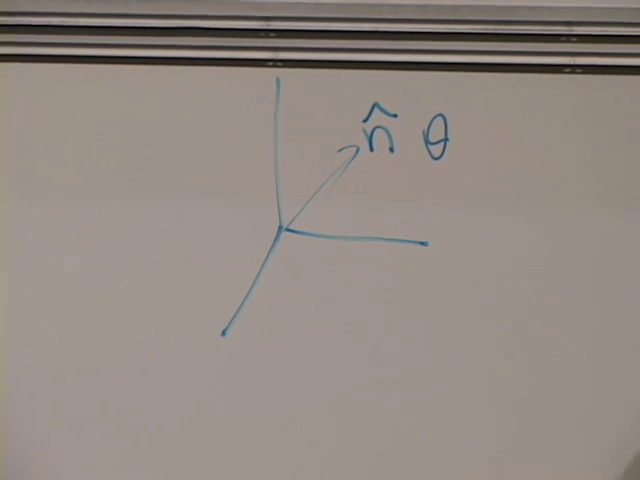
\includegraphics[width=0.58\textwidth]{lecture_03_figure_02.png}\caption{Un eje \(\hat{\boldsymbol n}\) y un ángulo \(\theta\) especifican una rotación espacial.}\lectureframe{00:02:34}\end{figure}

Una dirección sobre la esfera unidad requiere dos parámetros, como la longitud y la latitud. El ángulo alrededor de esa dirección aporta un tercero. Por tanto, las rotaciones forman una familia de tres parámetros. Por ahora no nos ocuparemos de las identificaciones globales debidas a ángulos que difieren en \(2\pi\); aquí importa el número local de parámetros.

La descripción mediante eje y ángulo tiene cierta redundancia. Invertir el eje e invertir el ángulo da la misma operación, y los ángulos suficientemente grandes pueden reducirse módulo una vuelta completa. Nada de esto cambia el hecho de que, cerca de la identidad, una rotación tiene tres parámetros que varían continuamente. Más adelante compararemos ese número local con el de parámetros independientes de una representación matricial.

Las propiedades de grupo pueden comprobarse una por una:
\begin{enumerate}
\item \emph{Clausura.} Realizar dos rotaciones sucesivas produce otra rotación.
\item \emph{Identidad.} La operación de no hacer nada es la rotación identidad.
\item \emph{Inverso.} Una rotación de ángulo \(\theta\) alrededor de \(\hat{\boldsymbol n}\) se deshace mediante una rotación de ángulo \(-\theta\) alrededor del mismo eje.
\item \emph{Asociatividad.} Tres rotaciones sucesivas satisfacen
\[
(R_1R_2)R_3=R_1(R_2R_3).
\]
\end{enumerate}

Las rotaciones no son conmutativas. En general, una rotación alrededor del eje \(x\) seguida de otra alrededor del eje \(y\) produce una orientación distinta de la que resulta al realizar las mismas dos operaciones en orden inverso:
\begin{equation}
R_x(\alpha)R_y(\beta)\ne R_y(\beta)R_x(\alpha).
\end{equation}
La diferencia es de segundo orden cuando ambos ángulos son muy pequeños; por eso las rotaciones infinitesimales pueden parecer casi conmutativas. Aun así, el grupo completo no es abeliano.

La falta de conmutatividad puede comprobarse sin ecuaciones. Tomen un libro o una caja, marquen una cara como frente y gírenlo noventa grados alrededor del eje \(x\) y luego noventa grados alrededor del eje \(y\). Vuelvan a la orientación inicial e inviertan el orden. La cara marcada acaba apuntando en otra dirección. Con ángulos pequeños, la discrepancia es más difícil de apreciar, pero no desaparece: comienza en el producto de los dos ángulos pequeños.

\begin{classroomqa}\audiencequestion{¿Estas rotaciones son sucesivas, en lugar de simultáneas?\lecturetimestamp{00:04:45}}\lecturerresponse{Sí. La multiplicación de grupo significa realizar una operación y luego otra. El orden de esas rotaciones sucesivas es precisamente lo que puede impedir la conmutatividad.}\end{classroomqa}

Este es nuestro primer grupo no abeliano. La aplicación que nos interesa finalmente no es el color de un objeto ordinario, sino los estados de color rojo, verde y azul de un quark. Se trata de un sistema interno de tres estados, cuyas transformaciones interesantes mezclan los tres colores. Las rotaciones ordinarias ofrecen un modelo familiar de cómo un grupo continuo actúa mediante matrices.

Un grupo por sí solo es abstracto. Para usarlo en física, debemos especificar sobre qué objetos actúa. Una {representación} asigna un operador o una matriz a cada elemento del grupo, de modo que el producto de elementos del grupo se reproduzca mediante el producto de las matrices asignadas. Distintos objetos físicos pueden tener distintas representaciones del mismo grupo. Los vectores y los estados de espín uno y de espín un medio serán tres ejemplos.

\section{La representación vectorial tridimensional}

Sea un vector ordinario de componentes
\begin{equation}
\boldsymbol V=(V_x,V_y,V_z),\qquad V_i,\quad i=1,2,3.
\end{equation}
Se puede rotar el vector físico manteniendo fijos los ejes, o rotar los ejes de coordenadas manteniendo fijo el vector. Las convenciones difieren, pero en ambas descripciones los componentes se mezclan mediante una matriz \(3\times3\). Para cada par de eje y ángulo \((\hat{\boldsymbol n},\theta)\), escribimos
\begin{equation}
V_i'=R_{ij}(\hat{\boldsymbol n},\theta)V_j,
\label{eq:l3-vector-rotation}
\end{equation}
donde se suma sobre los índices repetidos.

El índice repetido \(j\) es un índice mudo. La ecuación~\eqref{eq:l3-vector-rotation} significa explícitamente
\begin{equation}
V_i'=R_{i1}V_1+R_{i2}V_2+R_{i3}V_3
\end{equation}
para cada componente de salida \(i\). El índice libre \(i\) indica qué componente se calcula; se suma sobre el índice repetido \(j\), que puede cambiarse de nombre sin alterar la ecuación. Mantener separados estos dos papeles evita la mayoría de los errores de índices en el argumento de conservación de la longitud.

\begin{figure}[htbp]\centering
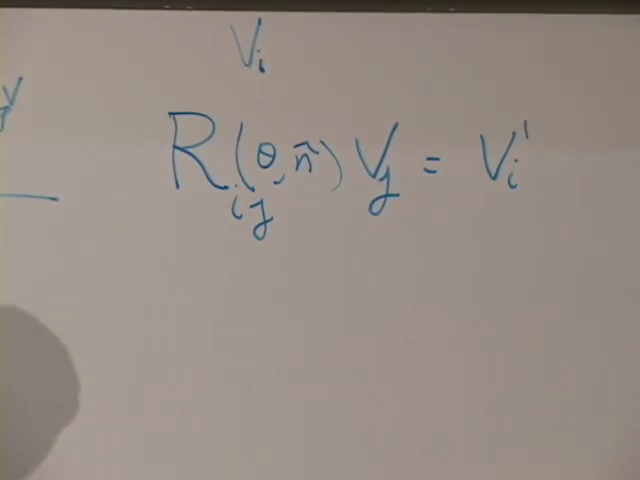
\includegraphics[width=0.68\textwidth]{lecture_03_figure_03.png}\caption{Una matriz de rotación transforma los componentes originales del vector en los componentes rotados.}\lectureframe{00:07:41}\end{figure}

Una rotación genuina conserva la longitud. Por ahora, tanto \(V_i\) como \(R_{ij}\) son reales, así que
\begin{equation}
V_i'V_i'=V_iV_i
\end{equation}
para cualquier vector. Para obtener la condición matricial, escribamos la misma transformación con índices mudos distintos:
\begin{equation}
V_i'=R_{ij}V_j,\qquad V_i'=R_{ik}V_k.
\end{equation}
Al multiplicar y sumar sobre \(i\), se obtiene
\begin{align}
V_i'V_i'
 &=R_{ij}V_jR_{ik}V_k\\
 &=R_{ij}R_{ik}V_jV_k.
\end{align}
Esto es igual a \(V_jV_j\) para cualquier elección de \(V\) solo si
\begin{equation}
R_{ij}R_{ik}=\delta_{jk}.
\label{eq:l3-orthogonality-index}
\end{equation}
En notación matricial,
\begin{equation}
R^TR=\boldsymbol 1,
\label{eq:l3-orthogonal}
\end{equation}
y, por tanto,
\begin{equation}
R^{-1}=R^T.
\end{equation}
La transposición simplemente intercambia las filas y las columnas.

¿Por qué el coeficiente debe ser \(\delta_{jk}\)? La delta de Kronecker fija \(j=k\) en la suma:
\begin{equation}
\delta_{jk}V_jV_k=V_1^2+V_2^2+V_3^2.
\end{equation}
Si \(R_{ij}R_{ik}\) fuera distinto de \(\delta_{jk}\), alguna dirección o algún término cruzado \(V_jV_k\) modificaría la longitud. Como la igualdad debe cumplirse para todo vector posible, y no solo para uno elegido, el coeficiente matricial debe ser la identidad.

La ecuación~\eqref{eq:l3-orthogonal} es la condición de ortogonalidad que define esta representación matricial real. El producto de las matrices reproduce la ley de composición de las rotaciones espaciales. Esta no es la única representación del grupo de rotaciones; simplemente es la más fácil de visualizar.

La relación del inverso tiene un significado geométrico inmediato. Se puede deshacer una rotación sin resolver una nueva ecuación matricial: basta intercambiar filas y columnas. Si \(R_1\) y \(R_2\) representan dos rotaciones, entonces \(R_2R_1\) representa su acción sucesiva y también es ortogonal. Así, las operaciones matriciales conservan la misma estructura de clausura, identidad, inverso y asociatividad establecida geométricamente.

\section{Espín uno y la representación vectorial}

La representación tridimensional también actúa sobre estados cuánticos. Una partícula de espín uno tiene tres proyecciones de espín posibles:
\begin{equation}
m=+1,\quad 0,\quad -1.
\end{equation}
Por tanto, su estado de espín es una columna de tres componentes formada por amplitudes de probabilidad. Al rotar la partícula, o al cambiar la orientación del campo magnético que define el eje de espín, esas tres amplitudes se mezclan mediante una representación tridimensional del grupo de rotaciones.

El número de estados de espín sigue la regla conocida \(2s+1\). El espín cero tiene un estado, el espín un medio tiene dos, el espín uno tiene tres y el espín tres medios tiene cuatro. Por tanto, la dimensión del vector de estado cambia con el espín. La misma rotación física debe representarse mediante matrices de tamaños distintos cuando actúa en esos diferentes espacios de estados.

Para una partícula de espín uno, elijamos la base
\begin{equation}
\lvert 1,+1\rangle,qquad
\lvert 1,0\rangle,qquad
\lvert 1,-1\rangle.
\end{equation}
Un estado es
\begin{equation}
\lvert\psi\rangle
=c_{+}\lvert1,+1\rangle+c_0\lvert1,0\rangle+c_{-}\lvert1,-1\rangle.
\end{equation}
Al rotar el aparato no se crea un cuarto estado de espín; los tres coeficientes \(c_+,c_0,c_-\) se mezclan entre sí. Por tanto, el operador de rotación correspondiente debe ser una matriz \(3\times3\).

Para el espín uno, esta representación se transforma igual que un vector espacial ordinario. Ese es el significado preciso de llamar \emph{partícula vectorial} a una partícula de espín uno: sus tres amplitudes de espín y las tres componentes de un vector obedecen la misma ley de rotación. No es necesario imaginar el estado cuántico como una flecha literal; la afirmación se refiere a cómo se mezclan sus componentes.

Esta correspondencia no es accidental. Un vector tridimensional y un estado de espín uno llevan representaciones tridimensionales equivalentes del grupo de rotaciones. La expresión {partícula vectorial} resume esa propiedad de transformación. No afirma que exista dentro de la partícula una diminuta flecha rígida que represente el estado de polarización cuántico.

\section{Simetrías discretas y continuas}

Antes de pasar al espín un medio, conviene distinguir dos grandes tipos de grupos. Una reflexión es un ejemplo discreto sencillo. Está la identidad y está la reflexión \(P\): o bien se invierte la orientación, o bien no. En cambio, una fase
\begin{equation}
e^{i\phi}
\end{equation}
depende continuamente de \(\phi\), y una rotación espacial depende continuamente de su eje y su ángulo. Estos grupos continuos se llaman \emph{grupos de Lie}, por Sophus Lie; el nombre se pronuncia \emph{«li»}. Las simetrías continuas serán nuestra principal preocupación, aunque las simetrías discretas también son importantes.

Para el grupo de dos elementos de reflexión,
\begin{equation}
P^2=1.
\end{equation}
no hay una cantidad de reflexión que pueda variarse continuamente entre \(1\) y \(P\). Un grupo de fases es distinto: entre \(e^{i\phi_1}\) y \(e^{i\phi_2}\) hay continuamente muchas otras fases. Las rotaciones espaciales tienen el mismo carácter continuo, pero, a diferencia de \(U(1)\), no son abelianas.

El espín cero da la representación más sencilla del grupo de rotaciones. Un estado de espín cero permanece inalterado bajo cualquier rotación, por lo que a cada elemento del grupo le corresponde la identidad unidimensional:
\begin{equation}
D^{(0)}(R)=1.
\end{equation}
El propio grupo sigue teniendo infinitas rotaciones; lo trivial es la representación sobre el estado de espín cero.

Es esencial distinguir entre un grupo y una de sus representaciones. El grupo de rotaciones no se reduce a un grupo de un solo elemento cada vez que actúa sobre un escalar. Más bien, cada uno de sus elementos se representa mediante el mismo número \(1\) en ese escalar particular.

\section{Un estado general de espín un medio}

Un sistema de espín un medio tiene dos estados de base. Respecto de un eje \(z\),
\begin{equation}
\lvert\uparrow\rangle=
\begin{pmatrix}1\\0\end{pmatrix},
\qquad
\lvert\downarrow\rangle=
\begin{pmatrix}0\\1\end{pmatrix}.
\end{equation}
Un estado general es un espinor de dos componentes:
\begin{equation}
\lvert\psi\rangle=
\begin{pmatrix}\alpha_1\\\alpha_2\end{pmatrix},
\qquad
|\alpha_1|^2+|\alpha_2|^2=1.
\label{eq:l3-spinor}
\end{equation}
Las entradas son complejas. La elección \((\alpha_1,\alpha_2)=(1,0)\) corresponde al espín hacia arriba, y \((0,1)\) al espín hacia abajo. Una combinación normalizada general describe un espín polarizado en alguna otra dirección.

Las palabras {arriba} y {abajo} solo tienen sentido una vez elegido un eje. Aquí, ese eje es \(z\). Un eje de medida distinto tiene otro par de estados de base, y un estado definido como arriba respecto de un eje suele aparecer como una superposición en otra base. Al rotar el espín físico o los ejes de referencia, los coeficientes cambian en consecuencia.

Dos amplitudes complejas contienen cuatro parámetros reales. La normalización elimina uno y la fase global físicamente irrelevante elimina otro, de modo que quedan dos parámetros reales. Ese es exactamente el número necesario para elegir una dirección sobre una esfera. Para estudiar las rotaciones no hace falta deducir la correspondencia explícita entre \((\alpha_1,\alpha_2)\) y esa dirección.

La fase global se elimina porque
\begin{equation}
\begin{pmatrix}\alpha_1\\\alpha_2\end{pmatrix}
\quad\hbox{and}\quad
e^{i\chi}
\begin{pmatrix}\alpha_1\\\alpha_2\end{pmatrix}
\end{equation}
representan el mismo rayo físico. La normalización fija la probabilidad total, no una dirección en el espacio euclidiano ordinario. Tras ambas identificaciones, los dos parámetros restantes pueden interpretarse como los ángulos polar y azimutal de la dirección de polarización del espín.

Al rotar el espín, su estado pasa a ser
\begin{equation}
\alpha_i'=U_{ij}\alpha_j,
\qquad
\begin{pmatrix}\alpha_1'\\\alpha_2'\end{pmatrix}
=
\begin{pmatrix}
U_{11}&U_{12}\\
U_{21}&U_{22}
\end{pmatrix}
\begin{pmatrix}\alpha_1\\\alpha_2\end{pmatrix}.
\label{eq:l3-spinor-transform}
\end{equation}
Así, las rotaciones espaciales tienen una representación matricial bidimensional que actúa sobre espinores. En esta representación hay una ambigüedad global de dos valores que dejaremos para más adelante; localmente, las matrices tienen las propiedades de transformación que necesitamos a continuación.

El par transformado \((\alpha_1',\alpha_2')\) debe seguir siendo un estado cuántico posible. Por tanto, la primera pregunta sobre \(U\) no se refiere a su fórmula explícita en función del eje y el ángulo, sino a la condición de que conserve la normalización de cualquier espinor de entrada.

\section{Conservación de la probabilidad y matrices unitarias}

Una rotación debe transformar un estado normalizado en otro estado normalizado:
\begin{equation}
\alpha_i^*\alpha_i=\alpha_i'^*\alpha_i'=1.
\end{equation}
Al sustituir la ecuación~\eqref{eq:l3-spinor-transform},
\begin{align}
\alpha_i'^*\alpha_i'
 &=(U_{ij}\alpha_j)^*(U_{ik}\alpha_k)\\
 &=\alpha_j^*U_{ij}^*U_{ik}\alpha_k.
\end{align}
se obtiene para los vectores reales la condición análoga
\begin{equation}
(U^T)^*U=\boldsymbol 1.
\end{equation}
La transposición seguida de la conjugación compleja es la conjugada hermítica:
\begin{equation}
U^\dagger=(U^T)^*,
\end{equation}
Por tanto, la condición de conservación de la normalización es
\begin{equation}
U^\dagger U=\boldsymbol 1.
\label{eq:l3-unitarity}
\end{equation}

La conjugación compleja adicional es el único cambio esencial respecto del cálculo con vectores reales. Para un vector real, \(V_iV_i\) es una longitud. Para un espinor, \(\alpha_i^*\alpha_i\) es una probabilidad. Se necesita la conjugación compleja para que esa probabilidad sea real y no negativa, así que la transposición se sustituye por la conjugada hermítica.

La ecuación~\eqref{eq:l3-unitarity} también da inmediatamente el inverso:
\begin{equation}
U^{-1}=U^\dagger.
\end{equation}
Por tanto, la rotación inversa conserva la misma norma de probabilidad. Al igual que las matrices de rotación ordinarias, los productos de matrices unitarias siguen siendo unitarios, de modo que la representación respeta la multiplicación del grupo.

\begin{figure}[htbp]\centering
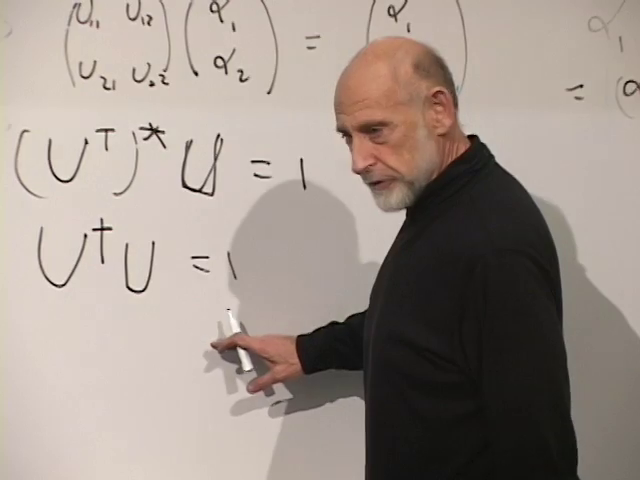
\includegraphics[width=0.62\textwidth]{lecture_03_figure_04.png}\caption{La matriz de rotación del espinor satisface \(U^\dagger U=\boldsymbol 1\).}\lectureframe{00:27:41}\end{figure}

Las matrices que satisfacen la ecuación~\eqref{eq:l3-unitarity} son unitarias. Una matriz compleja general \(2\times2\) comienza con ocho parámetros reales. La ecuación matricial de unitariedad \(2\times2\) impone cuatro restricciones reales independientes, con lo que quedan cuatro parámetros. Una rotación espacial solo tiene tres. Hace falta una restricción más para aislar la representación espinorial de las rotaciones de todas las matrices de \(U(2)\).

Las cuatro restricciones también pueden apreciarse al considerar las dos columnas de \(U\) como dos vectores complejos. Cada columna debe tener norma unitaria, lo cual aporta dos condiciones reales; además, las columnas deben ser ortogonales, lo cual aporta una condición compleja, o dos reales. En total, son cuatro. El cuarto parámetro restante en \(U(2)\) resultará ser una fase global del determinante, y no una nueva rotación espacial.

\section{Determinante uno y \texorpdfstring{\(SU(2)\)}{SU(2)}}

La condición adicional es
\begin{equation}
\det U=1.
\label{eq:l3-det-one}
\end{equation}
Es compatible con la multiplicación de grupo porque
\begin{equation}
\det(AB)=\det A\,\det B.
\end{equation}
El producto de dos matrices unitarias de determinante uno vuelve a tener determinante uno, y la identidad también tiene determinante uno. Estas matrices forman un subgrupo cerrado.

El inverso también pertenece al subgrupo. Si \(\det U=1\), entonces
\begin{equation}
\det U^{-1}=\frac{1}{\det U}=1.
\end{equation}
Así, imponer que el determinante sea uno no elimina la identidad, no rompe la clausura ni hace perder los inversos. Selecciona de forma coherente un grupo con un parámetro continuo menos.

La unitariedad por sí sola implica
\begin{equation}
\det(U^\dagger U)=
(\det U)^*\det U
=|\det U|^2=1.
\end{equation}
No obliga a que \(\det U\) sea \(+1\) o \(-1\). El determinante de una matriz unitaria general puede ser cualquier fase:
\begin{equation}
\det U=e^{i\phi},
\qquad
\det U^\dagger=e^{-i\phi}.
\end{equation}
La condición~\eqref{eq:l3-det-one} fija esa fase, que de otro modo sería libre, y elimina un parámetro real.

\begin{classroomqa}\audiencequestion{¿La condición \(U^\dagger U=\boldsymbol 1\), sin imponer que el determinante sea uno, obliga a que \(\det U^\dagger\) sea igual a \(\det U\) o a que solo pueda ser \(+1\) o \(-1\)?\lecturetimestamp{00:31:21}}\lecturerresponse{No. Los dos determinantes son complejos conjugados. Pueden ser \(e^{i\phi}\) y \(e^{-i\phi}\), cuyo producto es uno. La restricción de unitariedad especial obliga entonces a que ambos sean uno.}\end{classroomqa}

Las matrices unitarias \(n\times n\) forman \(U(n)\). Para \(n=1\), una matriz unitaria es simplemente la fase \(e^{i\phi}\), que da lugar a \(U(1)\). El subgrupo de determinante uno es el \emph{grupo unitario especial}:
\begin{equation}
SU(n)=\{U\in U(n):\det U=1\}.
\end{equation}
El espinor de dos componentes está sometido a la acción de \(SU(2)\), un grupo de tres parámetros.

La notación indica ambas restricciones: \(U\) significa unitario y \(S\) significa especial, es decir, de determinante uno. Estos grupos unitarios especiales aparecen repetidamente porque conservan un producto interno complejo y excluyen la fase común independiente que aporta el determinante.

Localmente, \(SU(2)\) tiene el mismo álgebra de rotaciones y la estructura de multiplicación necesaria para rotar estados de espín un medio. Globalmente, hay que recordar el matiz que dejamos pendiente: \(SU(2)\) es el recubrimiento doble del grupo de rotaciones ordinarias \(SO(3)\), así que dos elementos de \(SU(2)\) corresponden a una misma rotación espacial.\editorialnote{La formulación mediante el recubrimiento doble precisa la ambigüedad de dos valores mencionada, pero no desarrollada, en el texto original.}

\section{Rotaciones infinitesimales y matrices de Pauli}

\begin{classroomqa}\audiencequestion{¿Dónde aparecen en esta construcción las matrices de espín, o matrices de Pauli?\lecturetimestamp{00:33:16}}\lecturerresponse{Aparecen cuando se toma un elemento del grupo muy cerca de la identidad, lo que corresponde a una rotación de ángulo muy pequeño. Son los generadores de esas rotaciones infinitesimales.}\end{classroomqa}

Partamos de
\begin{equation}
U=\boldsymbol 1+\epsilon M+O(\epsilon^2),
\label{eq:l3-small-u-anti}
\end{equation}
donde \(\epsilon\) es real y pequeño. Entonces
\begin{equation}
U^\dagger=\boldsymbol 1+\epsilon M^\dagger+O(\epsilon^2),
\end{equation}
y la unitariedad da
\begin{align}
U^\dagger U
 &=\boldsymbol 1+\epsilon(M^\dagger+M)+O(\epsilon^2).
\end{align}
Al primer orden,
\begin{equation}
M^\dagger=-M.
\end{equation}
Así, la matriz \(M\) de la ecuación~\eqref{eq:l3-small-u-anti} es antihermítica.

Solo se conservan los términos lineales en \(\epsilon\). Se descarta el producto \(\epsilon^2M^\dagger M\) porque es de segundo orden. Esta es la ventaja de trabajar cerca de la identidad: las condiciones no lineales del grupo se convierten en condiciones lineales para sus generadores.

Es más conveniente extraer un factor de \(i\):
\begin{equation}
U=\boldsymbol 1+i\epsilon H+O(\epsilon^2).
\label{eq:l3-small-u-herm}
\end{equation}
La conjugación compleja transforma \(i\) en \(-i\), de modo que
\begin{equation}
U^\dagger=\boldsymbol 1-i\epsilon H^\dagger+O(\epsilon^2).
\end{equation}
Ahora,
\begin{equation}
U^\dagger U
=\boldsymbol 1+i\epsilon(H-H^\dagger)+O(\epsilon^2),
\end{equation}
y la unitariedad al primer orden exige
\begin{equation}
H^\dagger=H.
\end{equation}
Al dejar explícito el factor de \(i\), el generador resulta hermítico.

La multiplicación por \(i\) no ha cambiado las matrices infinitesimales permitidas; solo ha cambiado la convención para denominar el generador. En física se suelen elegir generadores hermíticos porque sus valores propios son reales y porque los observables asociados, como el momento angular, son hermíticos.

La condición de determinante uno implica que la traza sea nula.\editorialnote{El desarrollo verbal del determinante contiene un breve error en los subíndices. El término lineal corregido es \(A_{11}+A_{22}=\operatorname{tr}A\); los productos de elementos no diagonales empiezan en segundo orden.}. Para una matriz \(2\times2\) pequeña \(A\),
\begin{equation}
\det(\boldsymbol 1+A)
=
\det
\begin{pmatrix}
1+A_{11}&A_{12}\\
A_{21}&1+A_{22}
\end{pmatrix}.
\end{equation}
Al desarrollar,
\begin{align}
\det(\boldsymbol 1+A)
 &=(1+A_{11})(1+A_{22})-A_{12}A_{21}\\
 &=1+A_{11}+A_{22}+O(A^2)\\
 &=1+\operatorname{tr}A+O(A^2).
\end{align}
Al aplicar esto a \(A=i\epsilon H\),
\begin{equation}
\det U=1+i\epsilon\,\operatorname{tr}H+O(\epsilon^2).
\end{equation}
Por tanto, \(\det U=1\) exige
\begin{equation}
\operatorname{tr}H=0.
\end{equation}
La condición sobre la traza elimina precisamente el generador proporcional a la matriz identidad. Una matriz hermítica general \(2\times2\) tiene cuatro parámetros reales: dos elementos diagonales reales y un elemento no diagonal complejo. La traza fija una combinación real y deja tres parámetros. Esto coincide con los tres ejes alrededor de los cuales puede realizarse una rotación espacial infinitesimal.

Así pues, los generadores infinitesimales de \(SU(2)\) son matrices hermíticas \(2\times2\) de traza nula. Las tres matrices de Pauli forman una base:
\begin{equation}
\begin{aligned}
\sigma_x&=
\begin{pmatrix}0&1\\1&0\end{pmatrix},
&
\sigma_y&=
\begin{pmatrix}0&-i\\i&0\end{pmatrix},
\\[0.4em]
\sigma_z&=
\begin{pmatrix}1&0\\0&-1\end{pmatrix}.
\end{aligned}
\end{equation}
Todo generador puede escribirse
\begin{equation}
H=a_x\sigma_x+a_y\sigma_y+a_z\sigma_z.
\end{equation}
Una rotación pequeña alrededor del eje \(x\) selecciona \(\sigma_x\); una alrededor del eje \(y\) selecciona \(\sigma_y\); y una rotación alrededor de cualquier otro eje selecciona la combinación lineal correspondiente. En unidades en las que \(\hbar=1\), los operadores de espín son
\begin{equation}
S_i=\frac{\sigma_i}{2}.
\end{equation}

Por ejemplo, un eje a medio camino entre \(x\) y \(y\) usa un generador proporcional a
\begin{equation}
\frac{\sigma_x+\sigma_y}{\sqrt2}.
\end{equation}
La dirección del vector de coeficientes \((a_x,a_y,a_z)\) selecciona el eje de rotación, mientras que su magnitud, junto con \(\epsilon\), determina el ángulo pequeño. Esta es la conexión entre las matrices de espín que aparecen en los conmutadores de momento angular y los operadores de rotación finita. En particular,
\begin{equation}
[S_x,S_y]=iS_z
\end{equation}
y sus permutaciones cíclicas codifican la falta de conmutatividad que ya vimos geométricamente. La rotación finita estándar se obtiene al exponenciar el generador infinitesimal\editorialnote{La fórmula exponencial de la rotación finita completa la construcción infinitesimal de la forma habitual; la fuente solo deduce las condiciones para los generadores y su base de matrices de Pauli.}:
\begin{equation}
U(\hat{\boldsymbol n},\theta)
=\exp\left(-\frac{i\theta}{2}\,
\hat{\boldsymbol n}\cdot\boldsymbol\sigma\right).
\end{equation}\section{Un espacio de color de tres estados}

Podemos dejar para más adelante la combinación de representaciones. Ahora dejaremos atrás el espín espacial y volveremos al color de los quarks. Un quark sigue teniendo espín un medio, pero su color es un grado de libertad independiente de tres estados:
\begin{equation}
\lvert r\rangle,\qquad
\lvert g\rangle,\qquad
\lvert b\rangle.
\end{equation}
Un estado de color general es
\begin{equation}
\begin{aligned}
\lvert q\rangle_{\mathrm{color}}
={}&
\alpha_r\lvert r\rangle
+\alpha_g\lvert g\rangle
+\alpha_b\lvert b\rangle,
\\
&|\alpha_r|^2+|\alpha_g|^2+|\alpha_b|^2=1.
\end{aligned}
\end{equation}
Equivalentemente,
\begin{equation}
q=
\begin{pmatrix}
\alpha_r\\
\alpha_g\\
\alpha_b
\end{pmatrix}.
\end{equation}
Los módulos al cuadrado son las probabilidades de encontrar los colores rojo, verde y azul en una base de color elegida. La misma notación de triplete permite reunir tres operadores de campo de quark:
\begin{equation}
\psi=
\begin{pmatrix}
\psi_r\\
\psi_g\\
\psi_b
\end{pmatrix}.
\end{equation}

Hay que mantener conceptualmente separados el espín y el color. La etiqueta de espín indica cómo se transforma el estado bajo rotaciones del espacio físico. La etiqueta de color indica cómo se transforma bajo una simetría interna que no rota el laboratorio. Un estado de quark lleva ambas etiquetas, aunque en esta discusión se omite el espín para centrarnos en el color.

Escribir tres operadores de campo en una sola columna es más que una ayuda para organizar la información. Permite expresar la simetría mediante una sola ecuación matricial. Una transformación puede convertir un campo rojo en una combinación lineal de campos rojos, verdes y azules, del mismo modo que una rotación espacial convierte una componente de un vector en una combinación lineal de sus otras componentes.

Primero podemos imaginar transformaciones discretas que intercambian dos colores. La simetría más amplia contiene mezclas continuas de los tres. Una matriz de intercambio sencilla puede requerir una fase adicional para que su determinante sea uno; así, el intercambio queda incorporado en el grupo unitario especial.

Para dos estados de base, el intercambio simple se representa mediante
\begin{equation}
X=
\begin{pmatrix}0&1\\1&0\end{pmatrix},
\qquad
\det X=-1.
\end{equation}
Al multiplicar toda la matriz por \(i\), se obtiene
\begin{equation}
\det(iX)=i^2\det X=1.
\end{equation}
Por tanto, con una elección coherente de la fase, el intercambio discreto puede aparecer como un elemento particular del grupo continuo más amplio.

\begin{classroomqa}\audiencequestion{¿Una matriz que simplemente intercambia dos estados de base tiene un determinante inadecuado para \(SU(2)\)?\lecturetimestamp{00:43:46}}\lecturerresponse{El intercambio simple tiene determinante \(-1\). Un factor adecuado de \(i\) da una matriz representativa de determinante uno, de modo que el intercambio puede incluirse entre las transformaciones unitarias especiales continuas.}\end{classroomqa}

\section{\texorpdfstring{\(SU(3)\)}{SU(3)} y los ocho generadores de color}

La transformación continua de color es
\begin{equation}
\begin{aligned}
q'&=Uq,
&
U^\dagger U&=\boldsymbol 1,
\\
\det U&=1,
&
U&\in SU(3).
\end{aligned}
\label{eq:l3-su3-action}
\end{equation}
Las matemáticas son las mismas que en la construcción unitaria especial usada para espinores, pero ahora \(U\) es \(3\times3\). No se trata de una rotación del espacio físico, sino de una rotación en el espacio interno de color.

La unitariedad conserva la normalización del estado de color:
\begin{equation}
q^\dagger q
=|\alpha_r|^2+|\alpha_g|^2+|\alpha_b|^2.
\end{equation}
El determinante uno elimina la dirección de fase común \(U(1)\) del espacio de mezclas continuas. Las matrices resultantes pueden realizar intercambios sencillos, cambios de fase relativos y superposiciones genuinamente continuas, y todas pertenecen a un mismo grupo cerrado.

El número de parámetros se obtiene de inmediato. Una matriz compleja \(3\times3\) tiene nueve elementos complejos, es decir, dieciocho parámetros reales. La ecuación matricial \(U^\dagger U=\boldsymbol 1\) impone nueve condiciones reales. El determinante uno elimina una más:
\begin{equation}
\dim SU(3)=18-9-1=8.
\end{equation}
Así pues, \(SU(3)\) tiene ocho generadores infinitesimales independientes.

Las nueve condiciones reales de unitariedad también pueden entenderse considerando las columnas de \(U\). Tres columnas complejas deben tener cada una norma unitaria y, además, cada par debe ser ortogonal. Estas condiciones eliminan nueve de los dieciocho parámetros reales iniciales. La fase del determinante elimina el décimo y deja ocho. Este es el análogo para tres estados del recuento \(8-4-1=3\) correspondiente a \(SU(2)\).

La aparición del 8 es el mismo hecho que, en última instancia, da lugar a las 8 especies de gluones. Decir que no hay 9 gluones porque la restricción del determinante eliminó una dirección es solo una regla mnemotécnica. Con mayor precisión, las 9 matrices de color-anticolor se descomponen en una dirección singlete de color, proporcional a la identidad, y 8 direcciones sin traza. Los 8 generadores sin traza forman la estructura de color adjunta que portan los gluones de la QCD.\editorialnote{La formulación singlete más octete es la versión precisa estándar de la observación deliberadamente heurística de la fuente sobre el determinante; la construcción del campo gauge se desarrolla más adelante.}

En esta etapa, la relación con los 8 gluones es un anticipo, no una derivación completa. Para obtener partículas gauge, hay que promover la simetría de color a una simetría local y determinar los campos compensadores. Lo que ya ha mostrado el recuento de parámetros es que hay 8 direcciones independientes en las que una transformación de color \(SU(3)\) puede empezar a apartarse de la identidad.

\section{La simetría de color impone restricciones a la QCD}

La afirmación básica sobre la simetría es que la física permanece invariante bajo la transformación de color de la ecuación~\eqref{eq:l3-su3-action}. Esta es la simetría interna central de la cromodinámica cuántica. Mezclar las componentes de color es, en cuanto a su forma, análogo a mezclar las amplitudes de espín arriba y espín abajo; a su vez, esas transformaciones de espinor están relacionadas con rotaciones de direcciones espaciales, pero no deben confundirse estos tres espacios.

Decir que el color es una simetría significa que cambiar la base de color no altera las predicciones físicas. Rojo, verde y azul son nombres convenientes para tres vectores de base, no tres pigmentos observables. Una rotación simultánea \(SU(3)\) de las componentes de color debe dejar inalterada la forma de las leyes. Esta invariancia no es un rasgo estético opcional, sino el principio organizador de la QCD.

La simetría restringe el lagrangiano. En el ejemplo anterior de \(U(1)\), la invariancia bajo una transformación de fase común restringía los términos permitidos a aquellos que contenían factores equilibrados de un campo y su conjugado. En la QCD, del mismo modo, todos los términos deben ser invariantes bajo la transformación de color \(SU(3)\). Este requisito tiene consecuencias para las interacciones, las cantidades conservadas y la forma del campo de gluones.

Supongamos que un término propuesto tiene un índice de color libre. Bajo la ecuación~\eqref{eq:l3-su3-action}, ese índice rota, por lo que el término no puede ser invariante por sí solo. Los términos permitidos deben contraer los índices de color en combinaciones invariantes o usar campos gauge cuyas transformaciones compensen el cambio. Esta es la consecuencia práctica del principio de simetría: descarta acoplamientos arbitrarios y organiza las interacciones que sí se permiten.

La construcción completa de la QCD requiere un paso más: hay que permitir que la transformación de color varíe de un punto a otro, y el campo gauge debe compensar ese cambio local.\editorialnote{Localizar la simetría de color es la formulación gauge estándar de la discusión global de \(SU(3)\); esta lección de la fuente no desarrolla el tema.} Ese desarrollo corresponde a la etapa siguiente. Por ahora, la estructura esencial ya está establecida: un triplete de color sobre el que actúa una simetría unitaria especial de tres estados con 8 generadores.

Por el momento, el cálculo ha llegado tan lejos en la teoría de grupos como hace falta. Partimos de rotaciones que pueden representarse en el espacio ordinario, pasamos a las matrices que actúan sobre vectores y espinores, y luego aplicamos la misma lógica a un espacio interno de color. El siguiente paso puede volver a la física de partículas con el marco matemático ya disponible, en vez de exigirle al formalismo que sostenga por sí solo toda la explicación física.